

\documentclass[11pt]{article}
\usepackage[utf8]{inputenc}
\usepackage{geometry}
\usepackage{graphicx}
\usepackage{hyperref}
\usepackage{amsmath}
\usepackage{listings}
\usepackage{xcolor}
\usepackage{float}
\usepackage{subcaption}
\usepackage{algorithm}
\usepackage{algpseudocode}
\usepackage{booktabs} % For prettier tables
\usepackage{siunitx}

% Set page margins
\geometry{a4paper, margin=1in}

% Set up code listing style
\lstset{
    basicstyle=\ttfamily,
    commentstyle=\color{gray},
    keywordstyle=\color{blue},
    stringstyle=\color{red},
    showstringspaces=false,
    captionpos=b
}

\title{Diffusion models: M2 coursework report}
\author{Vishal Jain}
\date{\today}

\begin{document}

\maketitle

\tableofcontents

\newpage
\section{Background}
\subsection{Latent Variable Models}
Latent variable models are probabilistic models that model the probability distribution of the data $Pr(\mathbf{x})$ through the use latent variables $\mathbf{z}$. They define a joint distribution $Pr(\mathbf{x}, \mathbf{z})$ of the data $\mathbf{x}$ and an unobserved hidden / latent variable $\mathbf{z}$. They then describe $Pr(\mathbf{x})$ as a marginalisation of this joint probability over the latent variables:

$$
Pr(\mathbf{x}) = \int Pr(\mathbf{x}, \mathbf{z})dz.
$$

$$
Pr(\mathbf{x}) = \int Pr(\mathbf{x}|\mathbf{z}) Pr(\mathbf{z})dz.
$$
This is useful because relatively simple expressions for $Pr(\mathbf{x}|\mathbf{z})$ and $Pr(\mathbf{z})$ can define complex distributions $Pr(\mathbf{x})$. Typically, the distribution $Pr(\mathbf{x}|\mathbf{z})$ is approximated as a Gaussian with a fixed variance and a mean that given by a deep network of the latent variable $\mathbf{z}$. The distribution $Pr(\mathbf{z})$ is typically fixed to be a standard normal distribution.
$$
Pr(\mathbf{x}|\boldsymbol{\phi}) = \int Pr(\mathbf{x}, \mathbf{z}|\boldsymbol{\phi}) d\mathbf{z}
$$

$$
= \int Pr(\mathbf{x}|\mathbf{z}, \boldsymbol{\phi}) \cdot Pr(\mathbf{z}) d\mathbf{z}
$$

$$
= \int \text{Norm}_x [f(\mathbf{z}, \boldsymbol{\phi}), \sigma^2 \mathbf{I}] \cdot \text{Norm}_z [0, \mathbf{I}] d\mathbf{z} \quad
$$
The network is optimised using a variational bound of the log likelihood of the data, known as the Evidence Lower Bound (ELBO). In order to optimise the network, an encoder is defined which maps the data to the latent space and a decoder which maps the latent space to the data space. The encoder and decoder are trained jointly to maximise the ELBO. The details can be found in chapter 17 of Understanding Deep Learning by Simon Prince \cite{prince}.

Once the network is optimised, ancenstral sampling can be used to generate new samples. This involves sampling a latent variable $\mathbf{z^*}$ from the standard normal distribution and passing it through the decoder network to define the mean of the gaussian likelihood $Pr(\mathbf{x}|\mathbf{z})$. This is then sampled from to generate the new sample $\mathbf{x^*}$.

\subsection{Image Quality Metrics}
To evaluate the quality of the generated images, the following standard metrics are used:
\begin{itemize}
    \item Frechet Inception Distance (FID): measures the similarity between two sets of images by comparing the distance between two Gaussians fitted to their feature distributions \cite{Fid}. The features are found by passing the images through a pre-trained Inception network and extracting activations from a specific deep layer. A lower FID score suggests the generated images are more similar to the reference dataset.
    \item Mean Squared Error (MSE): A metric that measures the average squared difference between the pixel values of the generated and target images.
    \item Root Mean Squared Error (RMSE): The square root of the MSE, which provides a measure of the average difference between the pixel values of the generated and target images.
    \item Structural Similarity Index (SSIM): evaluates the similarity between two images, considering luminance, contrast, and structure \cite{ssim}. The score ranges from -1 to 1, where 1 denotes identical images and -1 signifies maximum dissimilarity.
    \item Peak Signal-to-Noise Ratio (PSNR): calculates the ratio between the maximum possible signal power and the power of corrupting noise that affects its representation. It is expressed in decibels (dB), with higher values indicating closer resemblance to the original image.
\end{itemize}
The FID scores are calculated using the \texttt{FrechetInceptionDistance} class from \texttt{torchmetrics} package. The relevant code is located in the \texttt{src/calc\_fid.py} script. The metrics SSIM and PSNR are calculated using the \texttt{piq} package, the relevant code is located in the \texttt{src/utils.py} script under the \texttt{calc\_image\_quality\_metrics} function.
% TODO: Make bold vectors consistent. Use \mathbf{} for all vectors.
\section{Introduction - Denoising Diffusion Probabilistic Models}
\subsection{Model Architecture}
% Provide a more continuous introduction following on from LVM, make it clear that we are discussing a specific type of LVM.
The denoising diffusion probabilistic model (ddpm) is a type of latent variable model where the encoder is predetermined and defines a discrete set of latent variables $\mathbf{z_1} \ldots \mathbf{z_T}$ of the same dimensionality as the data $\mathbf{x}$. The encoder defines a forward degradation process and the decoder describes the reverse denoising process. All the learnt parameters associated with the ddpm model are in the decoder network.

\subsubsection{Encoder}
The encoder takes as input an image $\mathbf{x}$ and outputs a latent (degraded) representation $\mathbf{z}$ through some degradation process. The implementation of the ddpm encoder in the original notebook degrades the input image $\mathbf{x}$ by gradually adding gaussian noise $\epsilon$ at each step $t$. It follows an update scheme:
\begin{equation}
    \begin{aligned}
        \mathbf{z_1} &= \sqrt{1-\beta_1} \cdot \mathbf{x} + \sqrt{\beta_1} \cdot \boldsymbol{\epsilon_1} \\
        \mathbf{z_t} &= \sqrt{1-\beta_t} \cdot \mathbf{z_{t-1}} + \sqrt{\beta_t} \cdot \boldsymbol{\epsilon_t} \quad \forall t \in 2, \ldots, T,
    \end{aligned}
    \end{equation}
    where $\epsilon_t \sim \mathcal{N}(0, I)$, $\beta_t \in [0,1]$ is the noise schedule, $T$ is the total number of steps and $z_t$ describes the latent representation at step $t$.

This is equivalent to the following update rule which can be used to calculate the latent variable $z_t$ directly from $x$:
\begin{equation}
    \mathbf{z_t} = \sqrt{\alpha_t} \cdot \mathbf{x} + \sqrt{1 - \alpha_t} \cdot \boldsymbol{\epsilon}, \quad \text{where } \alpha_t = \prod_{s=1}^{t} (1 - \beta_s).
    \label{eq:z_t_alpha}
\end{equation}

The implementation in the notebook uses the following linear schedule for $\beta_t$:
\begin{equation}
    \beta_t = \frac{t}{T}(\beta_{max}-\beta_{min})+ \beta_{min},
\end{equation}
where the default values are $\beta_{max} = 0.02$, $\beta_{min} = 0.0001$ and $T=1000$.

\subsubsection{Decoder}
The decoder takes as input a latent representation (noisy image) $z$, the current time step $\frac{t}{T}$ and outputs the noise which can be used to obtain the denoised image. The default decoder network in the notebook is structured as a convolutional neural network (CNN) with 5 layers, each configured to preserve the spatial dimensions of its input through the application of zero padding. The network architecture specifies a progression of feature channels as follows: it starts with an input of 1 channel, then expands to 16 channels in the first layer, increases to 32 channels through the second and third layers, contracts back to 16 channels in the fourth layer, and finally reduces to 1 channel in the fifth output layer. The first four convolutional layers use a 7x7 kernel size, while the final convolutional layer employs a 3x3 kernel, with all layers using a GELU activation function.

The decoder network also includes a fully connected network to calculate the time encodings, which is a high-dimensional representation of the scalar time step $\frac{t}{T}$. This involves generating a set of exponentially increasing frequencies to capture patterns at various scales, computing the sine and cosine for each time step across all frequencies to provide a cyclic representation of time that captures periodic patterns, and concatenating these sine and cosine values to form a unique time signature. This signature is then transformed through multiple linear layers, creating a high-dimensional representation of the scalar time step. This vector is reshaped so it can be broadcasted across the spatial domain of the feature map of the first layer in the CNN when added to it. This process effectively "informs" each spatial location in the feature maps about the current stage of the diffusion process, allowing the network to undo the appropriate amount of noise at each stage. The specific network used to learn the time encoding is a multi layer perceptron (MLP) with 2 hidden layers with 128 hidden units in each, the input layer takes the concatenated sine and cosine tensor of shape 32 (16*2) and the final layer outputs a tensor of size 16 - the number of channels output by the first convolutional layer in the CNN. All layers use a GELU activation function.

\subsection{Training Algorithm}
The optimal model parameters $\phi$ for the decoder network are by found by maximising the log likelihood of the training data $\{x_i\}_{i=1}^{I}$:
$$\hat{\boldsymbol{\phi}} = \arg\max_{\boldsymbol{\phi}} \left[ \sum_{i=1}^{I} \log \Pr(x_i | \boldsymbol{\phi}) \right] \quad$$
This is approximately equivalent to minimising the following loss function:
$$
L[\boldsymbol{\phi}] = \sum_{i=1}^{I} \sum_{t=1}^{T} \left\| g[\mathbf{z}_{it}, \frac{t}{T}; \boldsymbol{\phi}] - \boldsymbol{\epsilon}_{it} \right\|^2
$$
\begin{equation}
= \sum_{i=1}^{I} \sum_{t=1}^{T} \left\| g \left[\sqrt{\alpha_t} \cdot \mathbf{x}_i + \sqrt{1 - \alpha_t} \cdot \boldsymbol{\epsilon}_{it}, \frac{t}{T}; \boldsymbol{\phi} \right] - \boldsymbol{\epsilon}_{it} \right\|^2,
\label{eq:loss_function}
\end{equation}
where $g$ is the decoder network. The training algorithm works as follows: Loop over all batches in the current epoch, for every image in the batch randomly sample the current time step $t$ from a uniform distribution over the interval $[1, T]$. Then sample the noise $\boldsymbol{\epsilon}$ from a standard normal distribution. The latent representation $\boldsymbol{\mathbf{z}}_{t}$ is then calculated using the update rule given in equation \eqref{eq:z_t_alpha}. Input the latent variable $\boldsymbol{\mathbf{z}}_{t}$ and the time step fraction $\frac{t}{T}$ into the decoder network which then outputs the noise estimate $\hat{\boldsymbol{\epsilon}}$. Calculate the mean square error between the estimated noise and the true noise. Accumulate the losses over the entire batch and take a gradient step using the ADAM optimiser. Repeat for several epochs. This process is described in the pseudocode below:

\begin{algorithm}[H]
    \caption{Diffusion model training}
    \begin{algorithmic}[1]
    \State \textbf{Input:} Training data $x$
    \State \textbf{Output:} Model parameters $\boldsymbol{\phi}$
    \While{not converged} \Comment{Repeat until convergence}
        \For{$i \in \mathcal{B}$} \Comment{For every training example index in batch}
            \State $t \sim \text{Uniform}[1, \ldots, T]$ \Comment{Sample random timestep}
            \State $\boldsymbol{\epsilon} \sim \text{Norm}[0, \mathbf{I}]$ \Comment{Sample noise}
            \State $\boldsymbol{z}_{t} = \sqrt{\alpha_t} \cdot x_i + \sqrt{1 - \alpha_t} \cdot \boldsymbol{\epsilon}$ \Comment{Calculate latent variable}
            \State $\hat{\boldsymbol{\epsilon}} = g \left( \boldsymbol{z}_{t}, \frac{t}{T}; \boldsymbol{\phi}_t \right)$ \Comment{Estimate the noise}
            \State $\ell_i = \left\|\hat{\boldsymbol{\epsilon}} - \boldsymbol{\epsilon} \right\|^2$ \Comment{Compute individual loss}
        \EndFor
        \State Accumulate losses for batch and take gradient step
    \EndWhile
    \end{algorithmic}
\end{algorithm}
\subsection{Sampling}
It is clear from equation \ref{eq:z_t_alpha} that as $t$ increases, $Pr(\mathbf{z_t}|\mathbf{x})=Pr(\mathbf{z_t})=Norm_z[0,\mathbf{I}]$. Thus, to generate a new sample $\mathbf{x^*}$ ancestral sampling can be used. Where a latent variable $\mathbf{z_T^*}$ is sampled from the standard normal distribution and passed through the decoder network which denoises it to generate the new sample $\mathbf{x^*}$. In principle this can be done in one shot as the decoder estimates the total noise at each step. However, in practice better results are obtained by iteratively denoising and sampling the latent variable $z_{t-1}$ at step. The sampling algorithm is outlined below:

\begin{algorithm}
    \caption{Sampling Algorithm 18.2}
    \begin{algorithmic}[1]
    \State \textbf{Input:} Model $g$
    \State \textbf{Output:} Sample, $x$
    \State $z_T \sim \mathcal{N}(0, I)$ \Comment{Sample last latent variable}
    \For{$t = T$ \textbf{down to} $2$}
        \State $\tilde{z}_{t-1} \gets \frac{1}{\sqrt{1-\beta_t}} z_t - \frac{\beta_t}{\sqrt{1-\alpha_t}\sqrt{1-\beta_t}} g(z_t, \phi_t)$ \Comment{Predict previous latent variable}
        \State $\varepsilon \sim \mathcal{N}(0, I)$ \Comment{Draw new noise vector}
        \State $z_{t-1} \gets \tilde{z}_{t-1} + \sigma_t \varepsilon$ \Comment{Add noise to previous latent variable}
    \EndFor
    \State $x \gets \frac{1}{\sqrt{1-\beta_1}} z_1 - \frac{\beta_1}{\sqrt{1-\alpha_1}\sqrt{1-\beta_1}} g_{\theta_1}(z_1, \phi_1)$ \Comment{Generate sample from $z_1$ without noise}
    \end{algorithmic}
\end{algorithm}

\subsubsection{Choice of Hyperparameters}
To demonstrate some of the underlying assumptions behind diffusion models, the following runs vary the noise schedule.
Specifically, a constant noise schedule is used where $\beta_t = C, \ \forall t \in \{1,2,...,T\}$, where $C$ is a constant.
The value of C and the total number of steps $T$ are varied between runs. The first run uses a small value of $C$ and a large value of $T$, while the second run uses a large value of $C$ and a smaller value of $T$. The first run is expected to perform better as only a small amount of noise at each step. This is significant because one of the assumptions used to derive the loss defined by \ref{eq:loss_function} is that the reverse distributions $Pr(z_{t-1}|z_{t})$ are well approximated by a normal distribution. This approximation is only valid for small $\beta_t$.
\subsubsection{Training details}

The DDPM model detailed in the previous sections was trained on the MNIST dataset across 50 epochs, utilising two distinct constant noise schedules with parameters set at $\beta = 0.001, T=2000$ and $\beta=0.1, T=200$. The dataset was randomly split into training and validation sets using an 80:20 ratio. A normalisation was applied to map the data to the range $[-0.5, 0.5]$ via the \texttt{Normalize} transform from the \texttt{torchvision.transforms} module. The ADAM optimiser was used with a learning rate of $2 \times 10^{-4}$ and a batch size of 128.
\subsubsection{Training and Validation Loss Curves}
Figure \ref{fig:q1b_loss_curves} presents the loss curves for both training and validation for the two runs, illustrating the model's performance under each noise schedule configuration.
\begin{figure}[H]
    \centering
    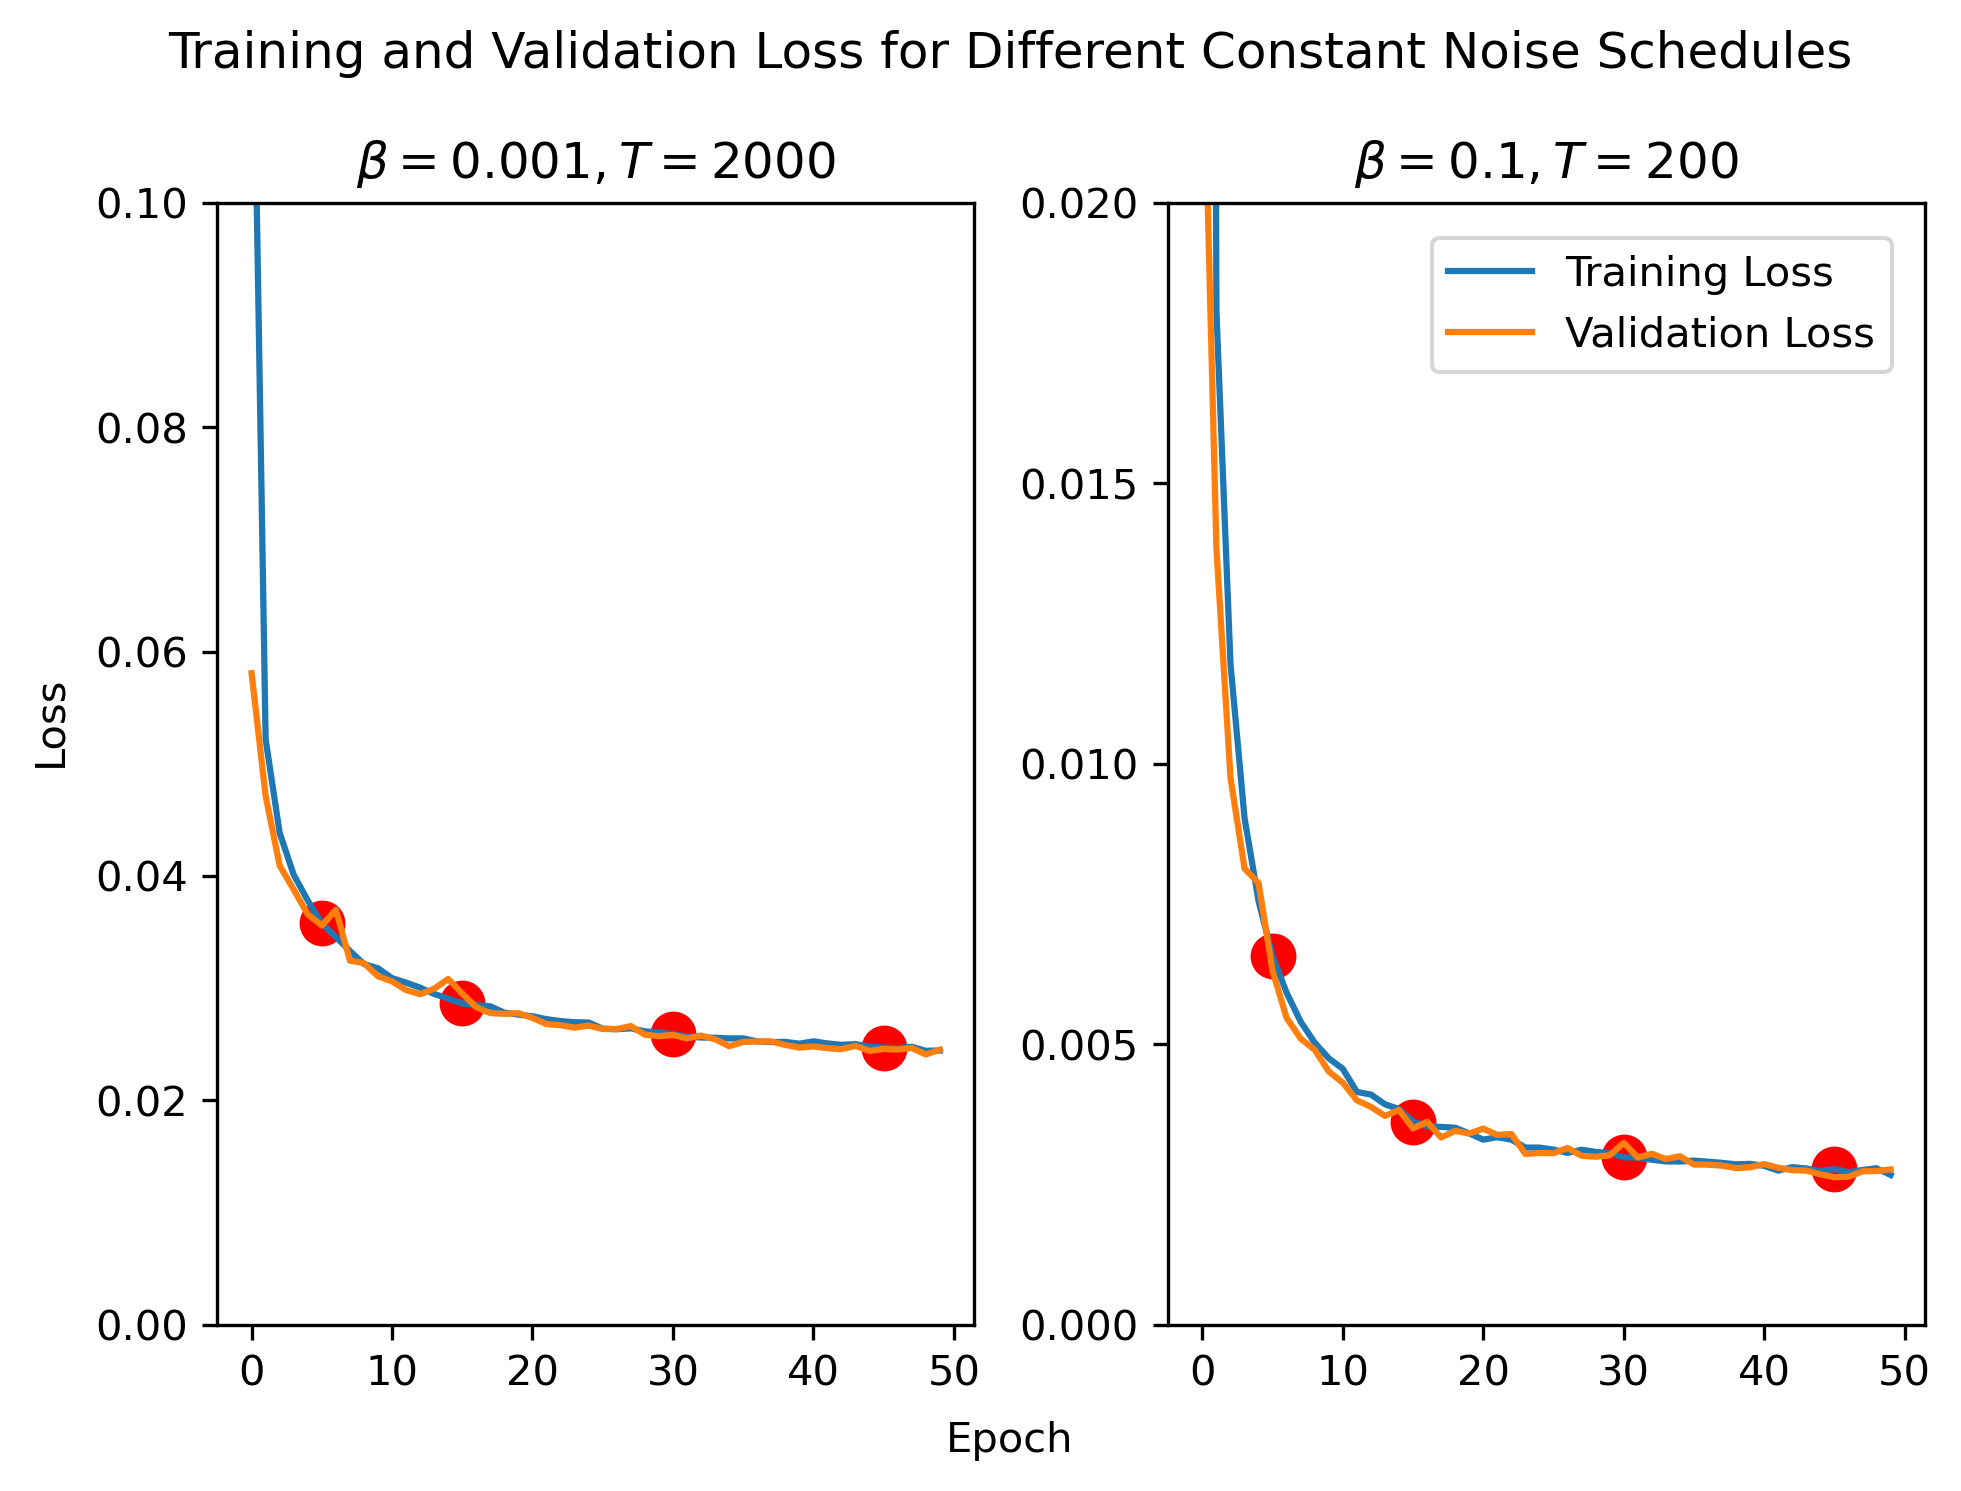
\includegraphics[width=0.8\textwidth]{figs/q1b_loss.png}
    \caption{Training and validation loss curves of the two runs. Training loss shown in blue, validation loss in orange. Red dots indicate epochs 5, 15, 30 and 45 at which the conditional and unconditionally generated samples are shown.}
    \label{fig:q1b_loss_curves}
\end{figure}

The validation loss curves follow the training loss curves closely, indicating that the model is not overfitting.
\subsubsection{Quality of samples}
From the loss curves alone it would appear that the larger $\beta$ model is performing better. However, the loss curves do not tell the whole story. Figures \ref{fig:train_conditional_samples} and \ref{fig:train_unconditional_samples} show the samples generated by the model at epochs 5, 15, 30 and 45. The samples generated by the model with the smaller $\beta$ value are of obviously of higher quality. Further, the model with the larger $\beta$ does not seem to be training well, with its conditional and unconditionally generated samples showing little improvement over the epochs. This is likely due to the fact that the reverse distributions $Pr(z_{t-1}|z_{t})$ are not well approximated by a normal distribution for large $\beta_t$ values as the noise added at each step is too large.

\begin{figure}[H]
    \centering
    \begin{minipage}{0.48\textwidth}
        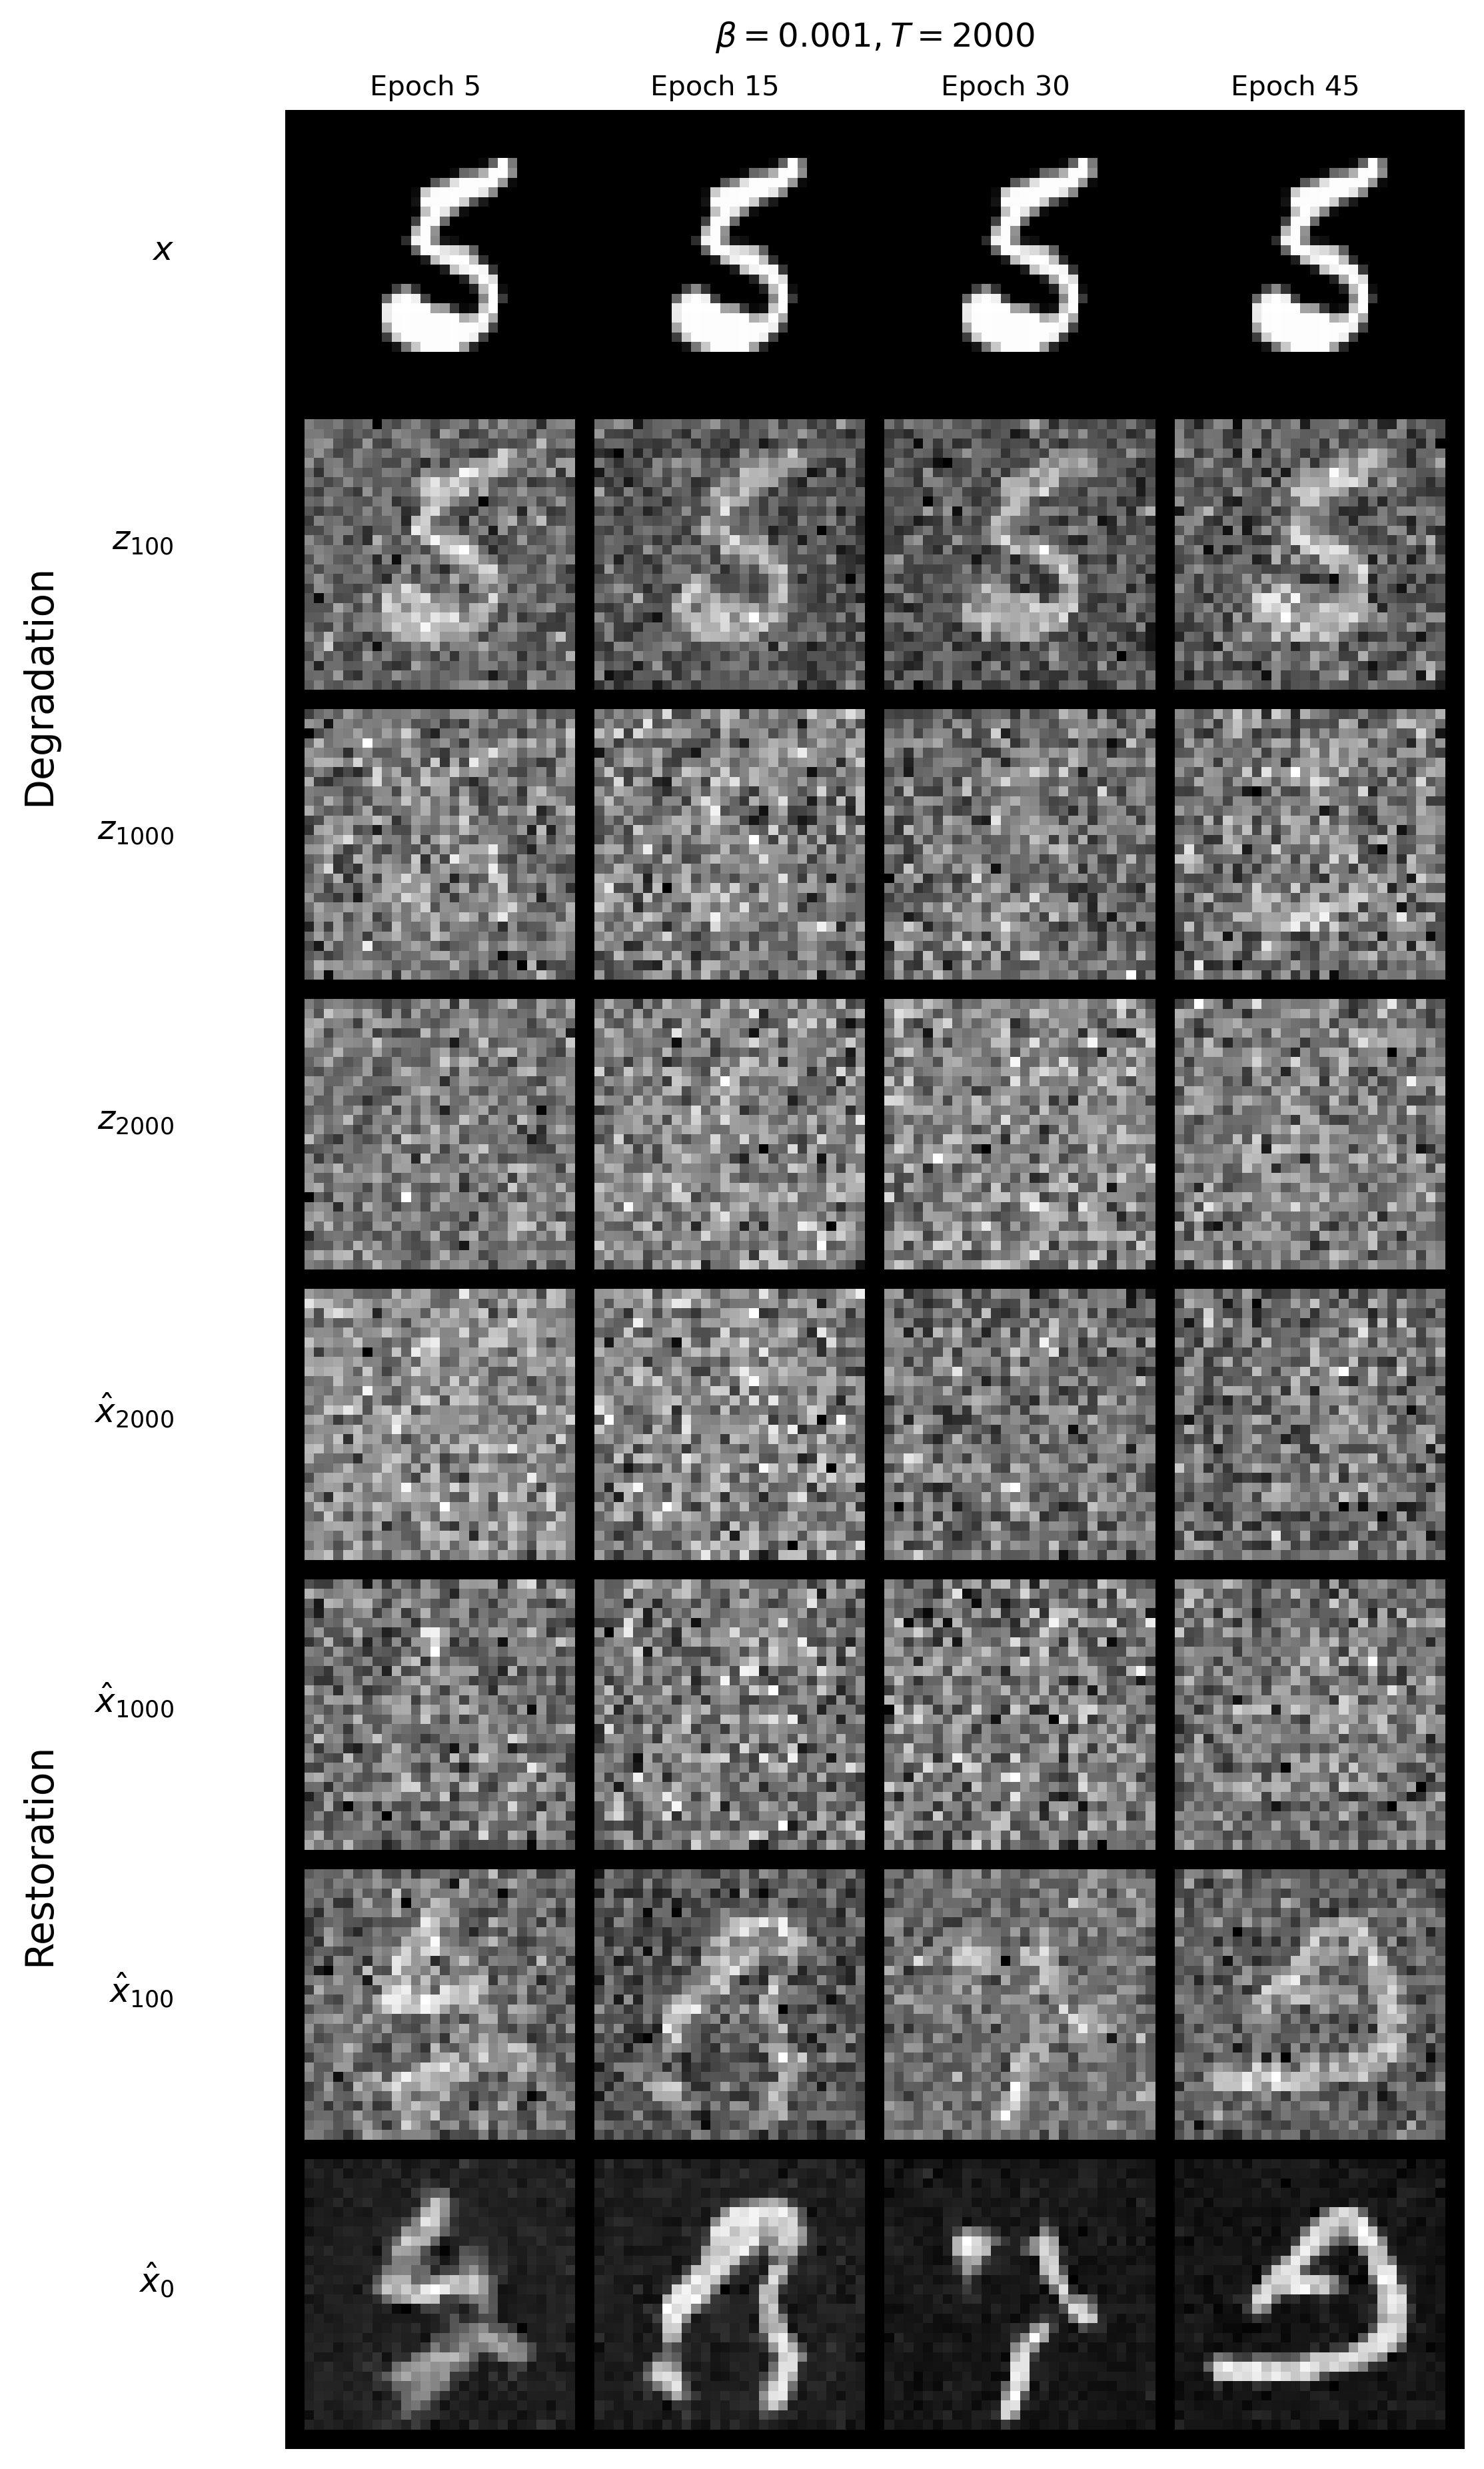
\includegraphics[width=\linewidth]{figs/q1b_good_cond_samples.png}
        \label{fig:train_cond_left_img}
    \end{minipage}\hfill
    \begin{minipage}{0.48\textwidth}
        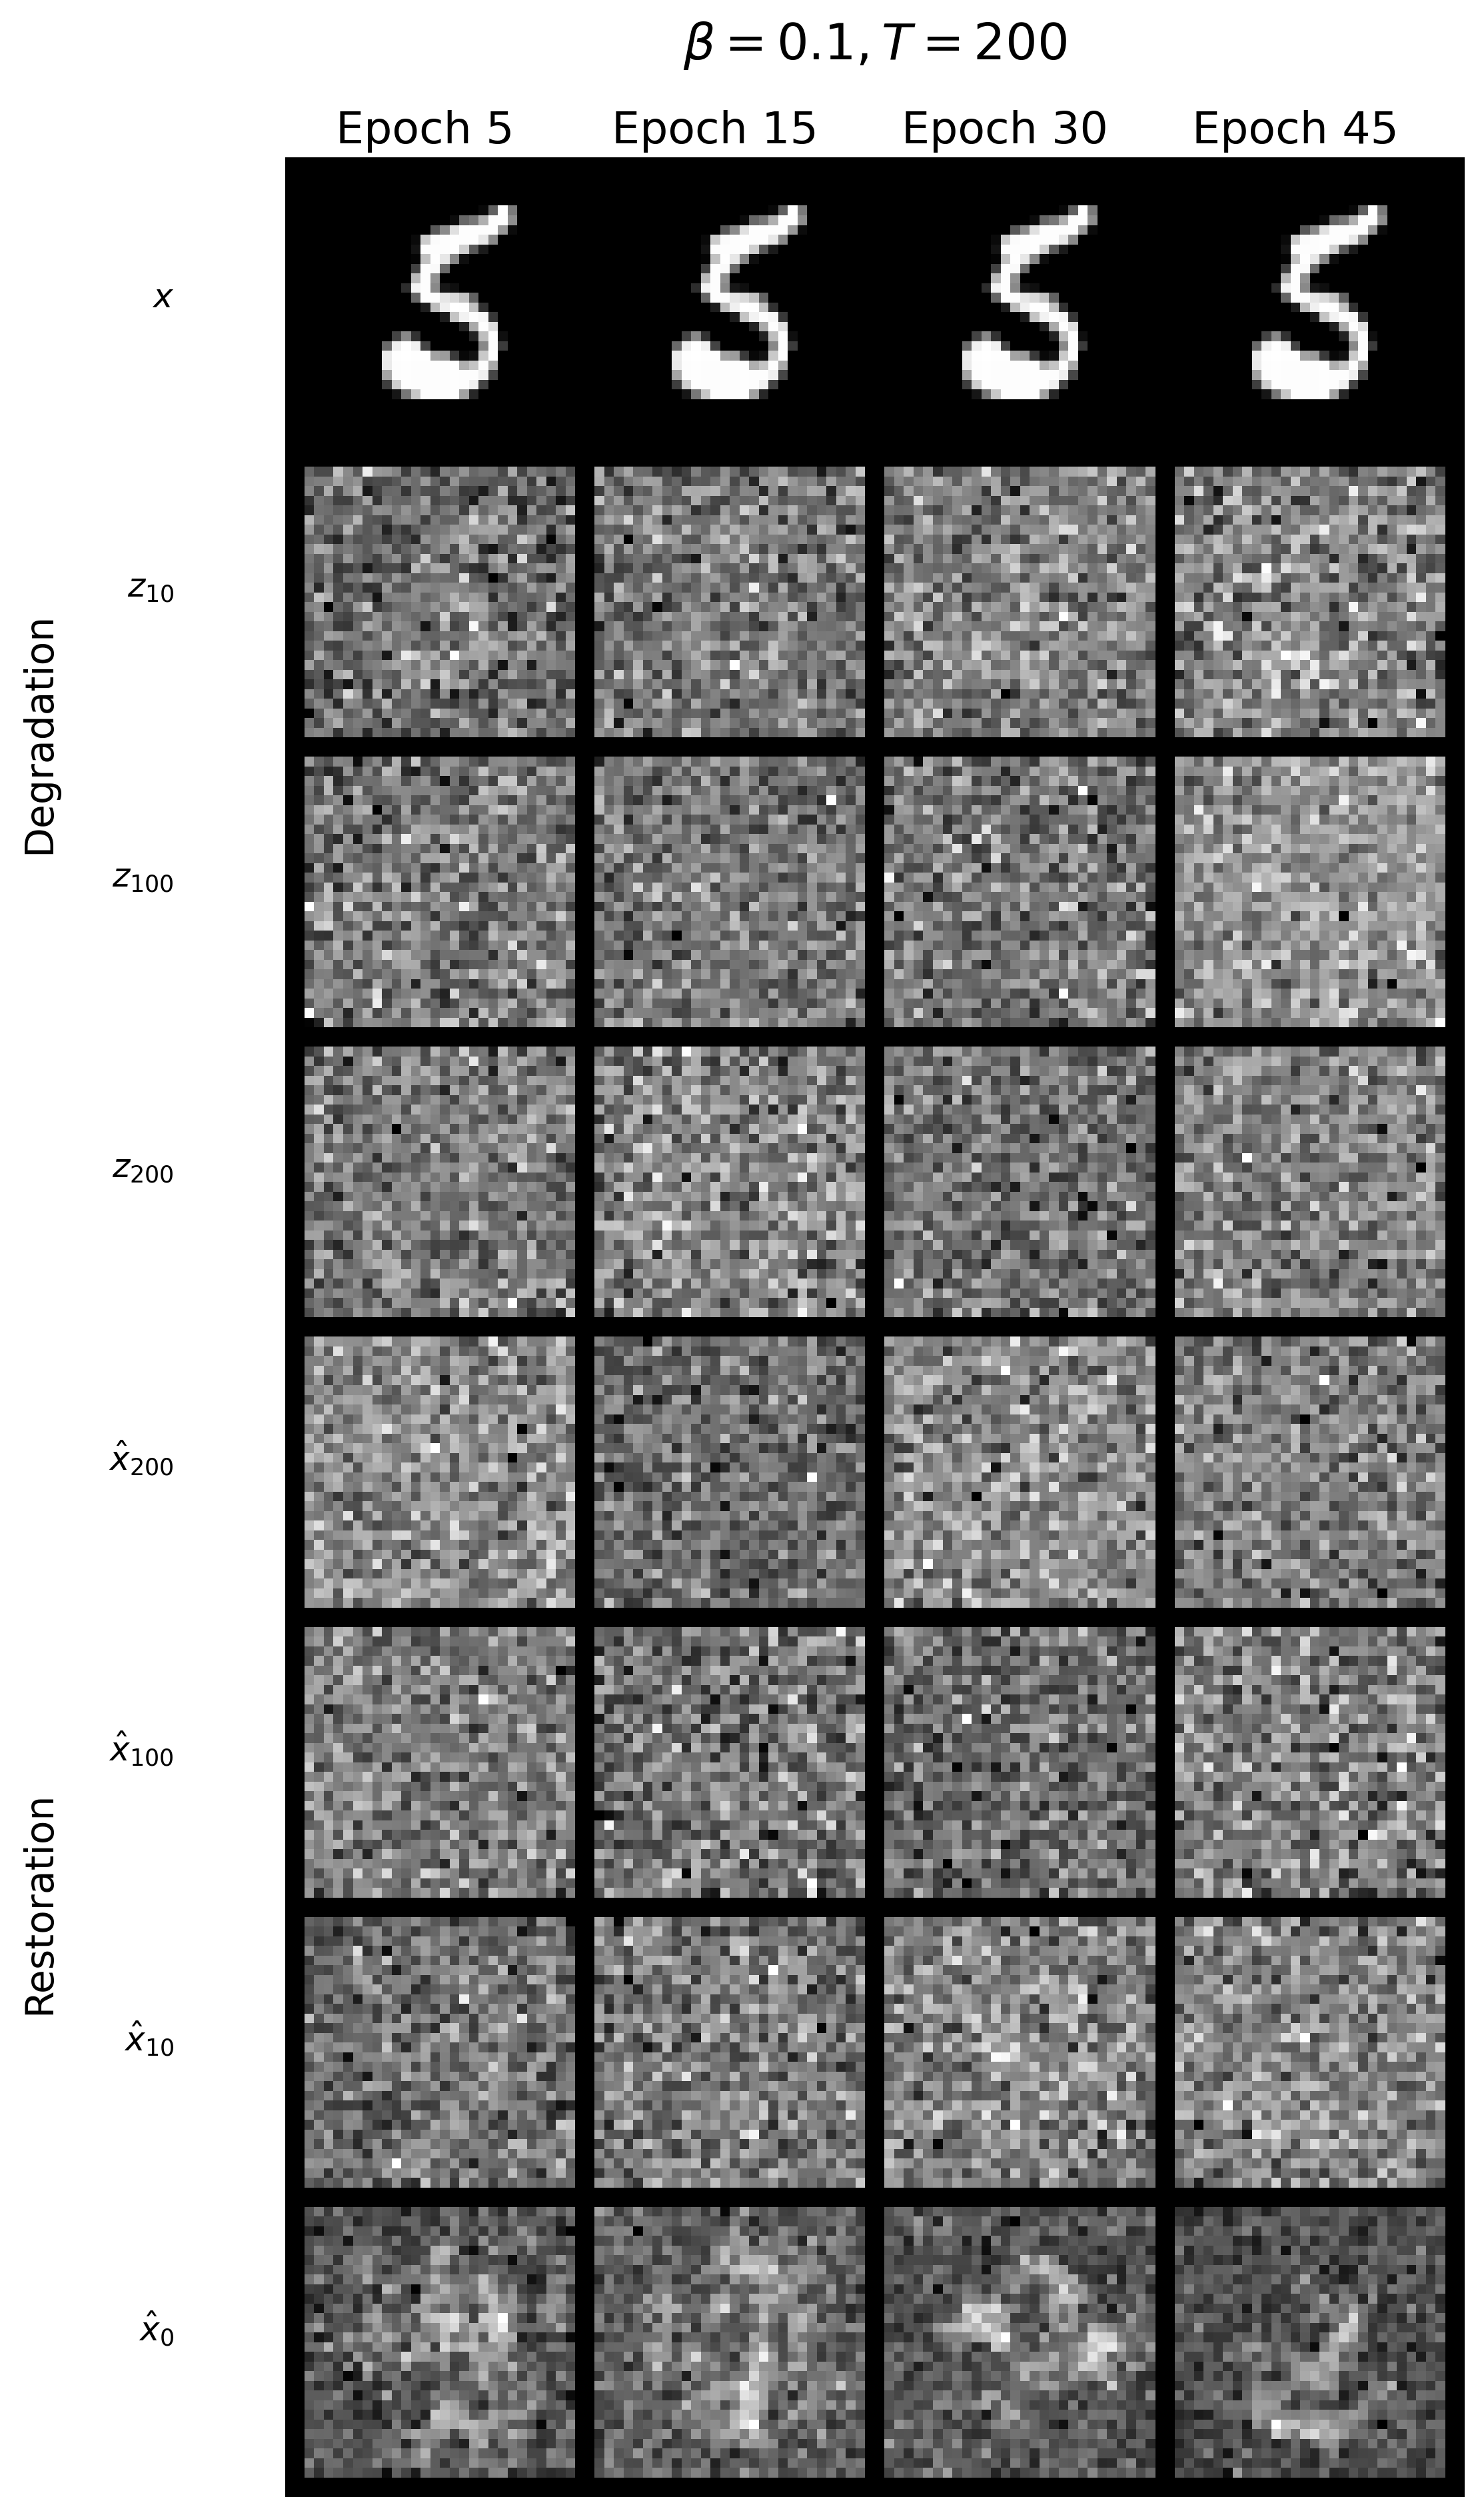
\includegraphics[width=\linewidth]{figs/q1b_bad_cond_samples.png}
        \label{fig:train_cond_right_img}
    \end{minipage}
    \caption{Conditionally generated samples as a function of epoch. $\beta=0.001, T=2000$ model shown on the left and $\beta=0.1, T=200$ shown on the right. The y axis shows the degraded latent variable $z_t$ at 3 times and the reconstructions denoted by $x_t$ at the same times along with the initial image $x$ (first row) and the final reconstructions $\hat{x}$ (last row).}
    \label{fig:train_conditional_samples}
\end{figure}

\begin{figure}[H]
    \centering
    \begin{minipage}{0.48\textwidth}
        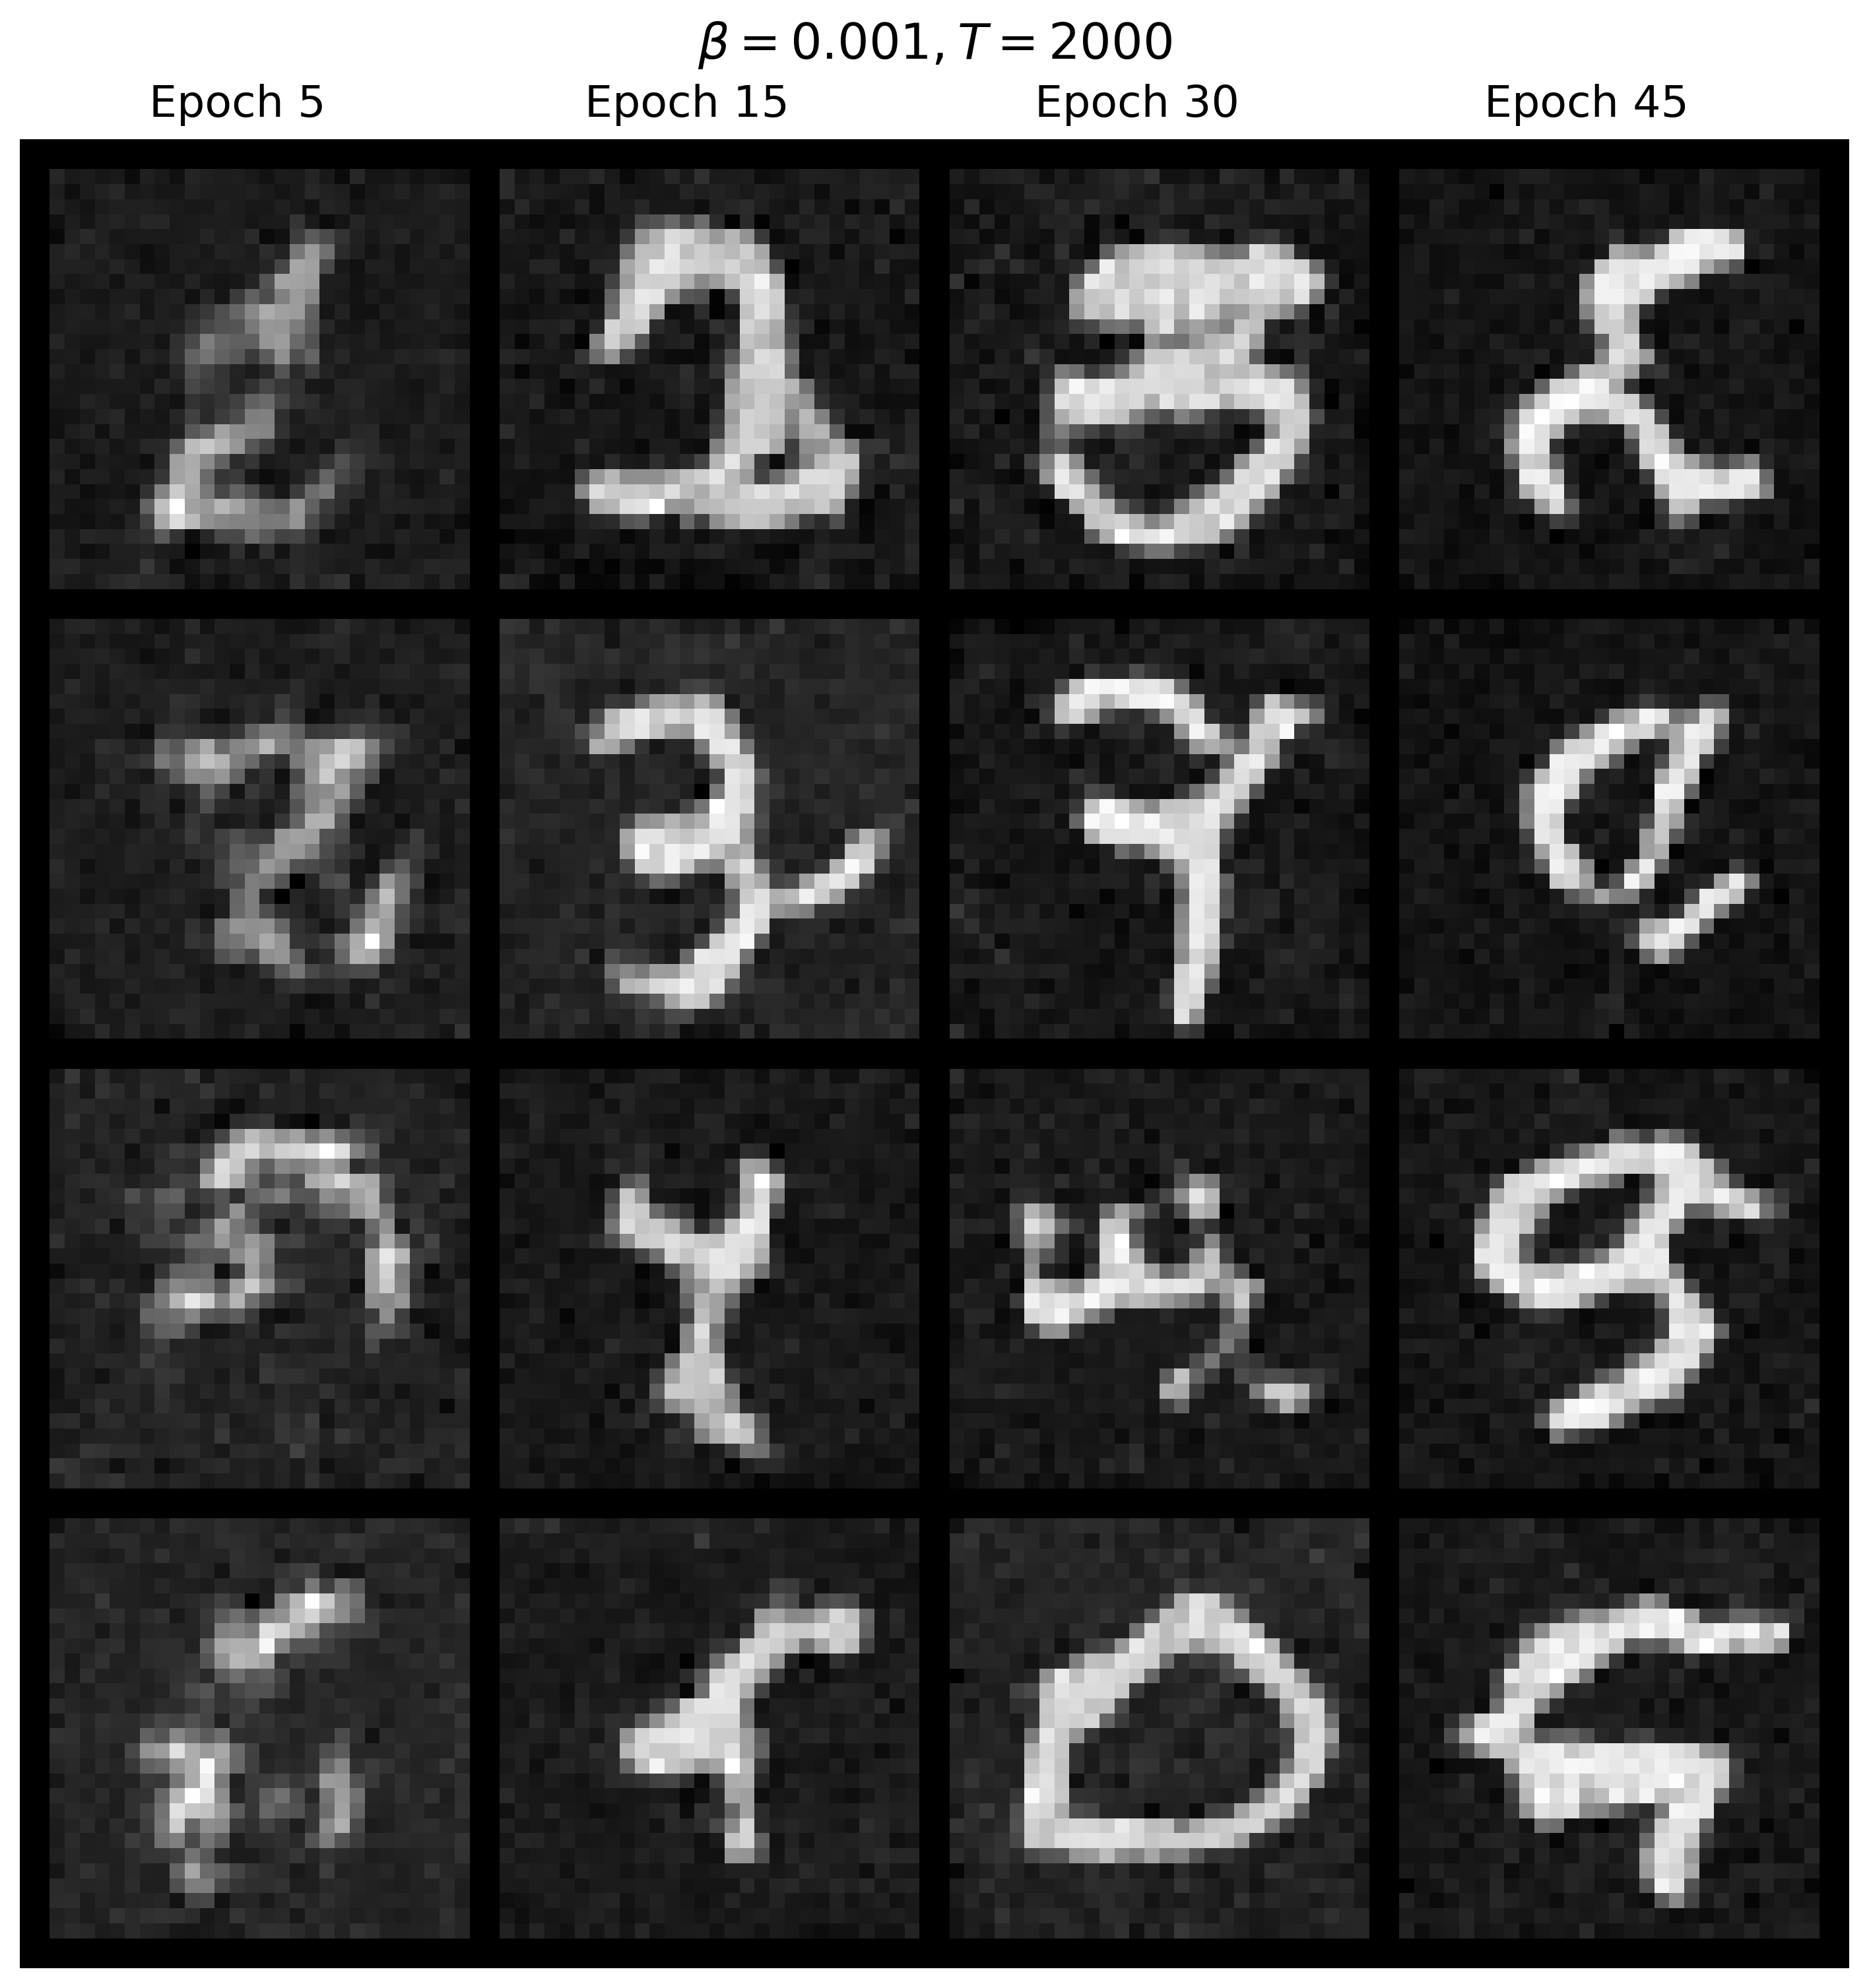
\includegraphics[width=\linewidth]{figs/q1b_good_uncond_samples.png}
        \label{fig:train_uncond_left_img}
    \end{minipage}\hfill
    \begin{minipage}{0.48\textwidth}
        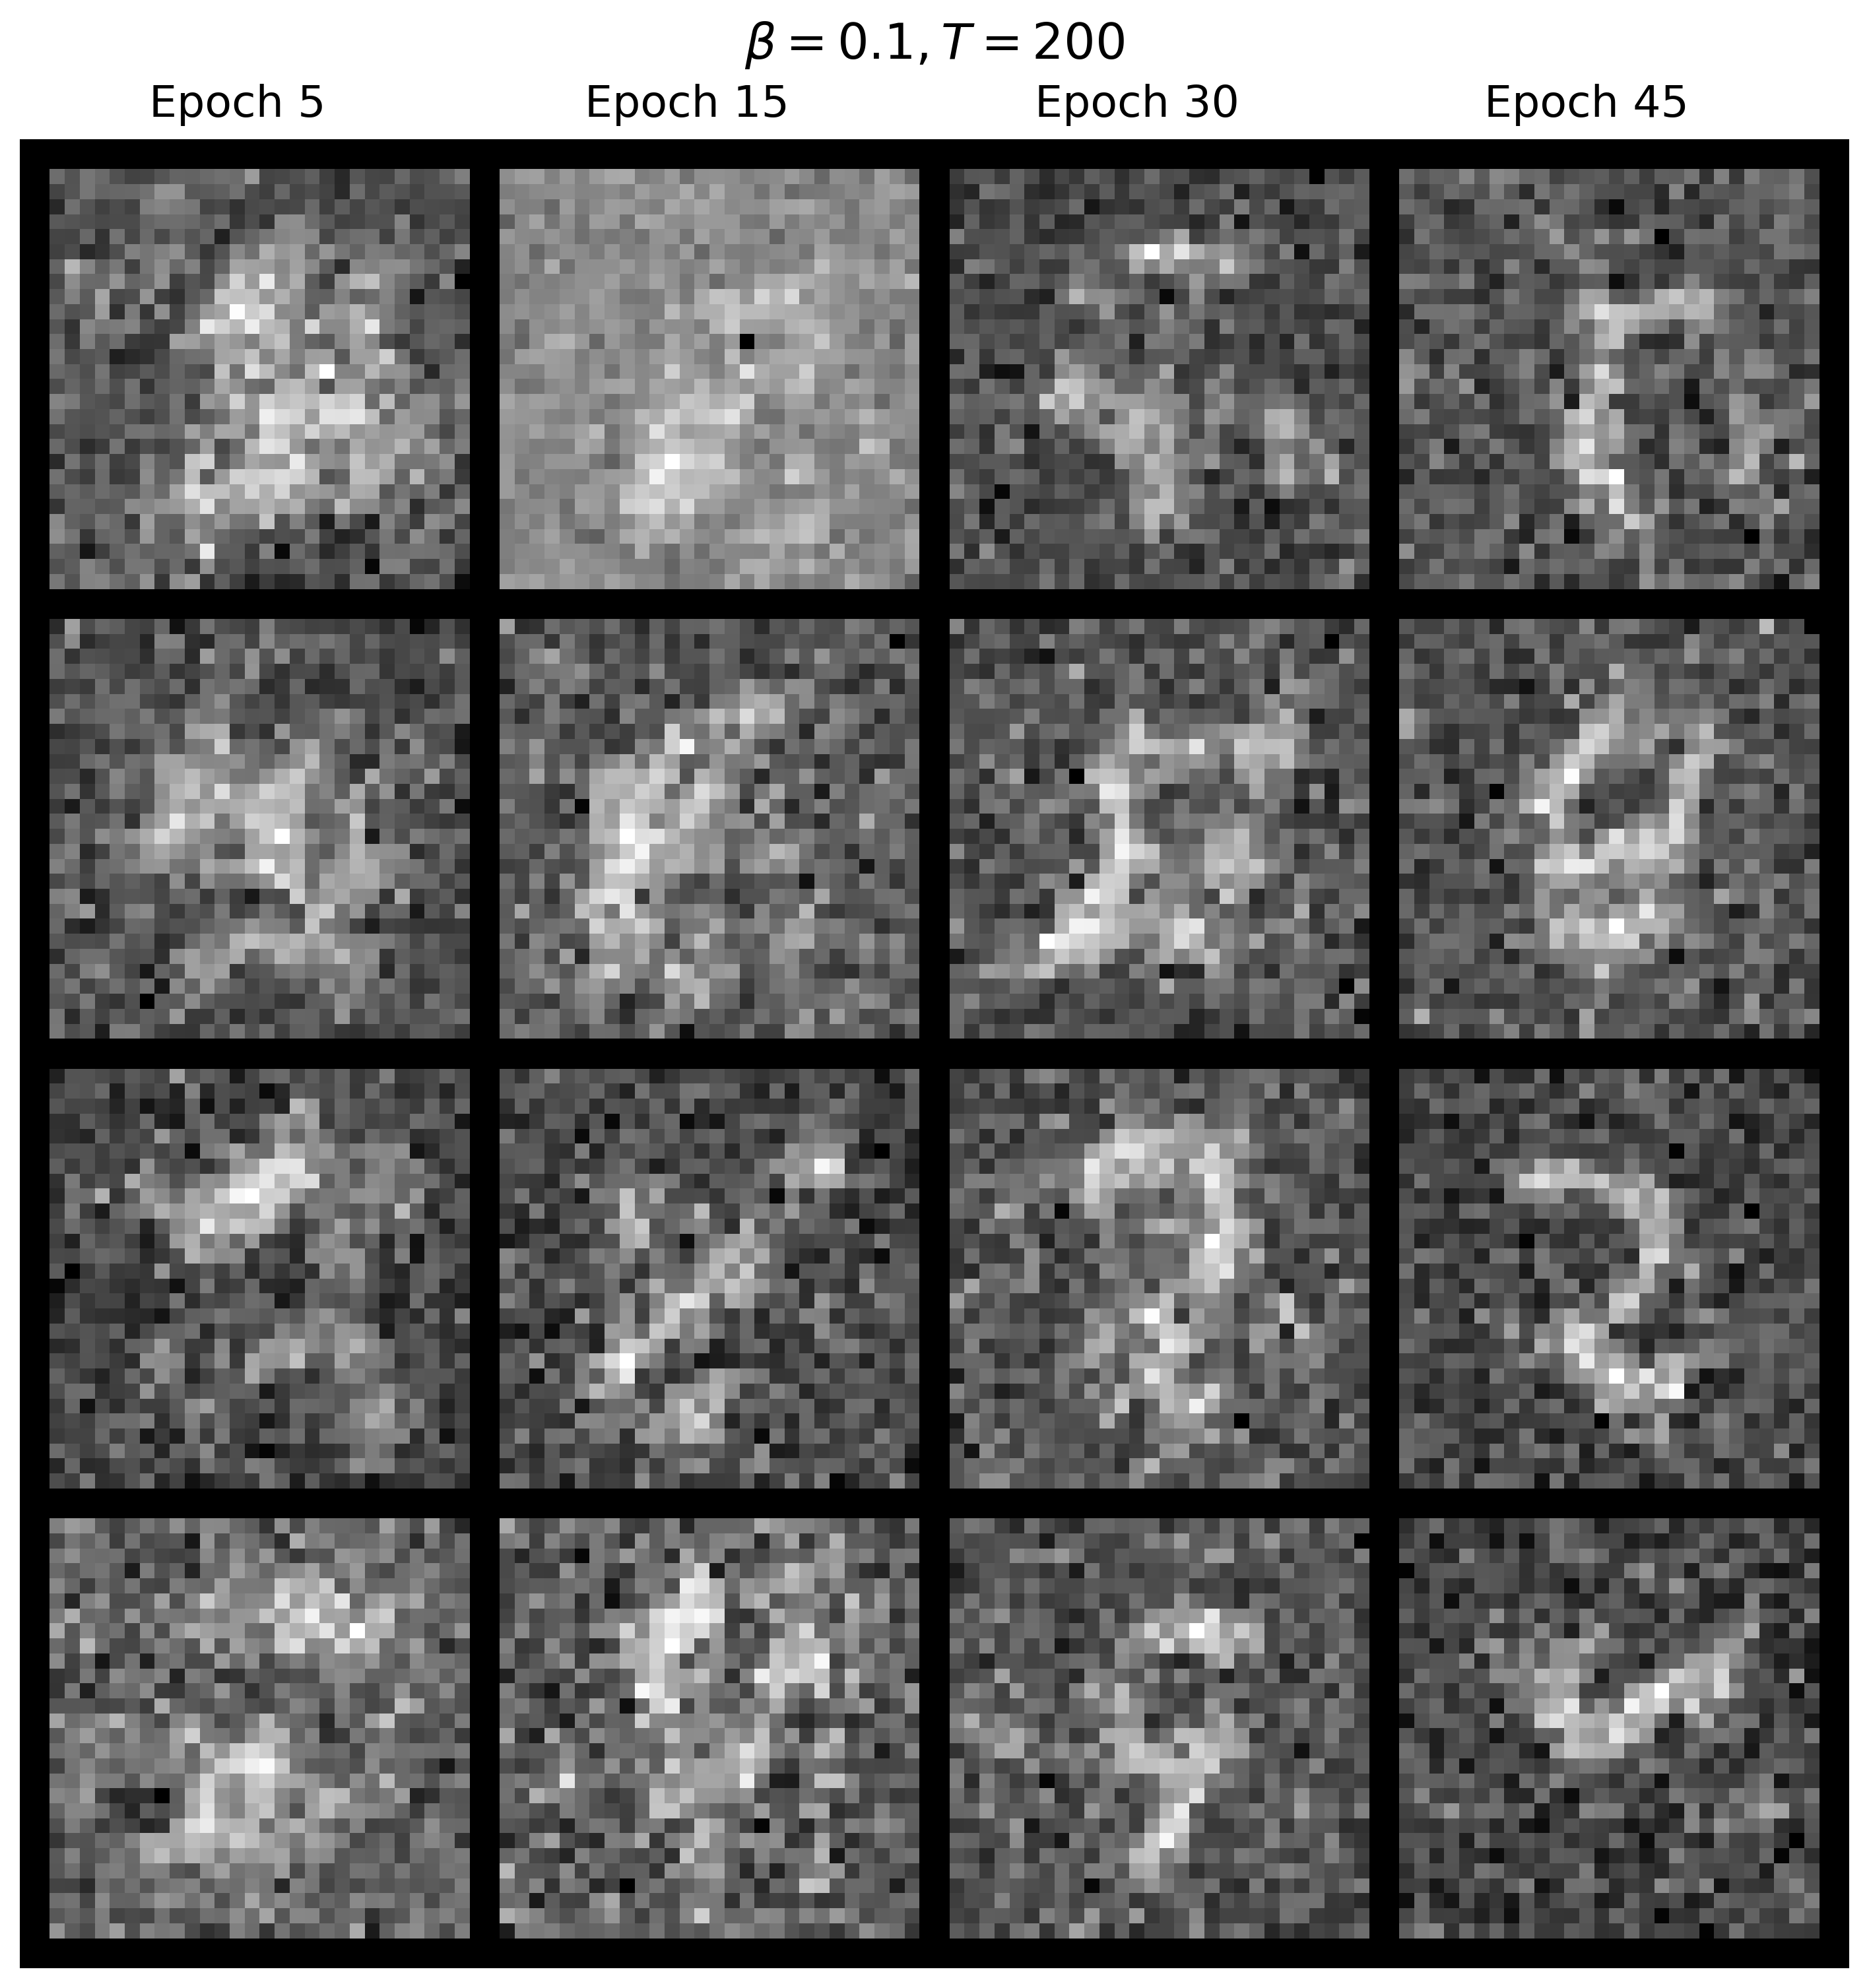
\includegraphics[width=\linewidth]{figs/q1b_bad_uncond_samples.png}
        \label{fig:train_uncond_right_img}
    \end{minipage}
    \caption{Unconditionally generated samples with the good $\beta=0.001$ value (left) and the bad $\beta=0.1$ value (right), shown as a function of the number of epochs.}
    \label{fig:train_unconditional_samples}
\end{figure}
\subsection{Evaluation}
The best model for each noise schedule was selected based on the validation loss and is compared for a final evaluation using the FID score, average test loss, average RMSE, average SSIM, and average PSNR. The results are summarised in the table \ref{tab:q1b_model_comparison} below. It is worth noting the FID score is calculated using unconditionally generated samples whereas the other metrics are evaluating using conditionally generated samples. Further, while the test loss shows the MSE between the estimated noise and the true noise, the other metrics compare the generated images directly with the images from the MNIST dataset. The FID scores are computationally expensive to calculate and so were calculated over a batch of 1000 samples. The other metrics were calculated over the entire test set of 10000 samples. For this reason the FID score is more noisy than the other metrics.
\begin{table}[H]
    \centering
    \caption{Comparison of Model Performances}
    \begin{tabular}{l|lllll}
    \hline
    Model          & FID Score           & Avg Test Loss        & Avg RMSE           & Avg SSIM         & Avg PSNR           \\ \hline
    Low $\beta$, High $T$ & \textbf{233}    & 0.0245              & \textbf{0.306}            & \textbf{0.164} & \textbf{10.5}    \\
    High $\beta$, Low $T$  & 432             & \textbf{0.00275}     & 0.402  & 0.0336          & 7.94              \\ \hline
    \label{tab:q1b_model_comparison}
    \end{tabular}
    \end{table}

    \begin{figure}[H]
        \centering
        \begin{minipage}{0.48\textwidth}
            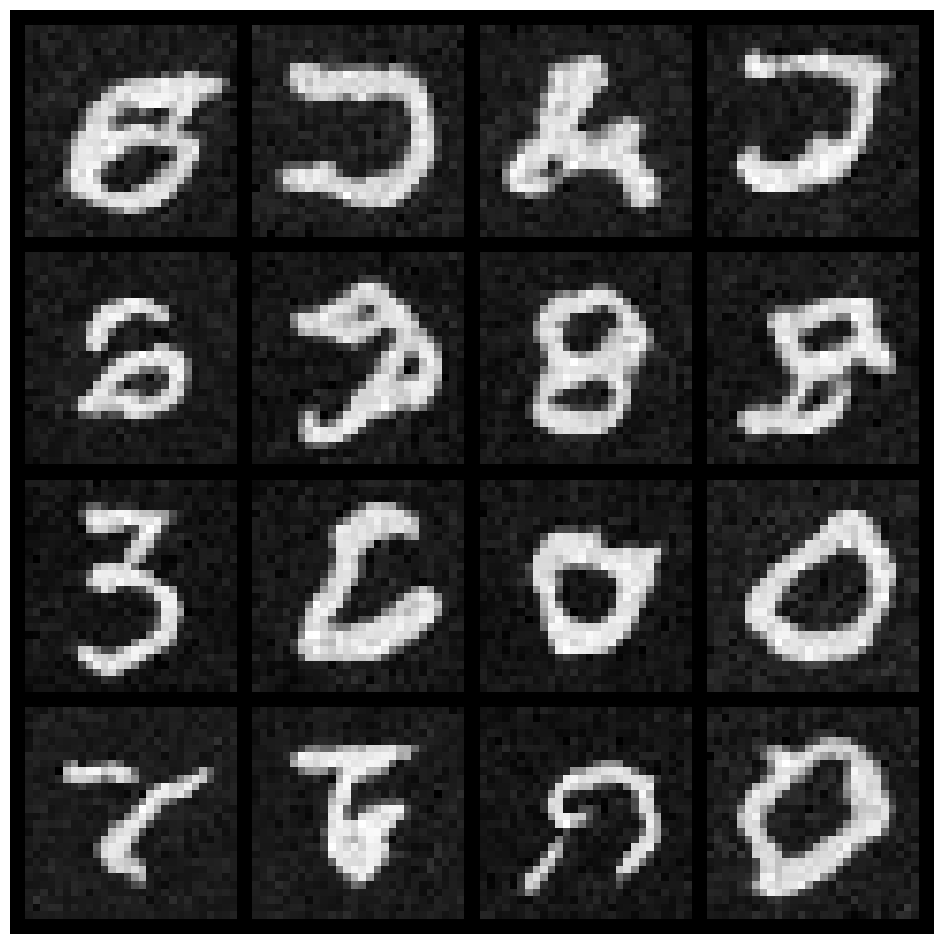
\includegraphics[width=\linewidth]{figs/q1c_good_uncond_samples.png}
            \label{fig:left_img_2}
        \end{minipage}\hfill
        \begin{minipage}{0.48\textwidth}
            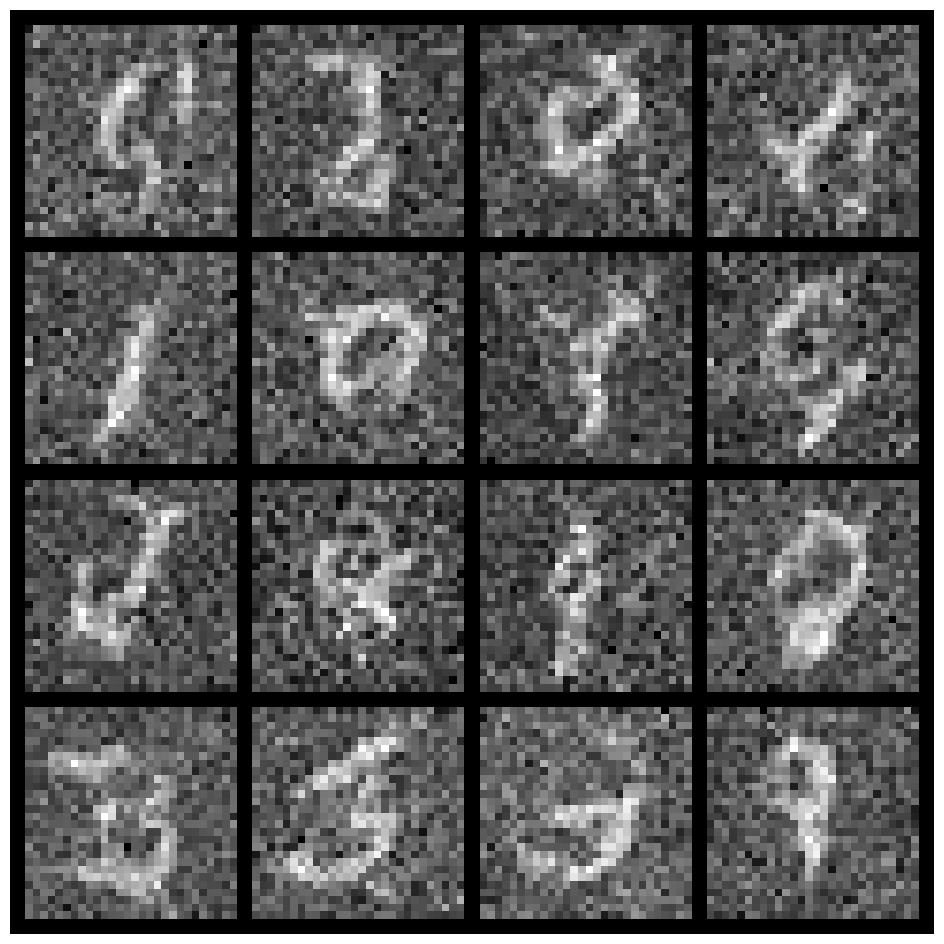
\includegraphics[width=\linewidth]{figs/q1c_bad_uncond_samples.png}
            \label{fig:right_img_2}
        \end{minipage}
        \caption{64 Unconditionally generated samples for the model $\beta = 0.001, T=2000$ (left) and the bad model  $\beta = 0.1, T=200$ (right).}
        \label{fig:q1c_unconditional_samples}
    \end{figure}

The model with the smaller $\beta$ value performs better across all metrics, with the exception of the average test loss. The FID score is significantly lower for the model with the smaller $\beta$ value, indicating that the generated samples are more similar to the reference dataset.  To further illustrate the differences between the two models, 64 samples are unconditionally generated and are shown in figure \ref{fig:q1c_unconditional_samples}. The samples generated by the model with the smaller $\beta$ value are of higher quality. Interestingly, the model with a higher $\beta$ value records a lower average test loss, a phenomenon that becomes clear when examining the noise schedules depicted in Figure \ref{fig:q1c_noise_schedules}. The rapid decay of $\alpha_t$ for the larger $\beta$ value significantly influences the latent variable $z_t$, primarily by the noise $\epsilon_t$. This leads the model to effectively disregard the input image $x$, opting instead to mimic the identity function and minimise the Mean Squared Error (MSE) without accurately learning the data's underlying distribution. This scenario underscores that a lower test loss is not always indicative of meaningful learning or enhanced model performance.

\begin{figure}[H]
    \centering
    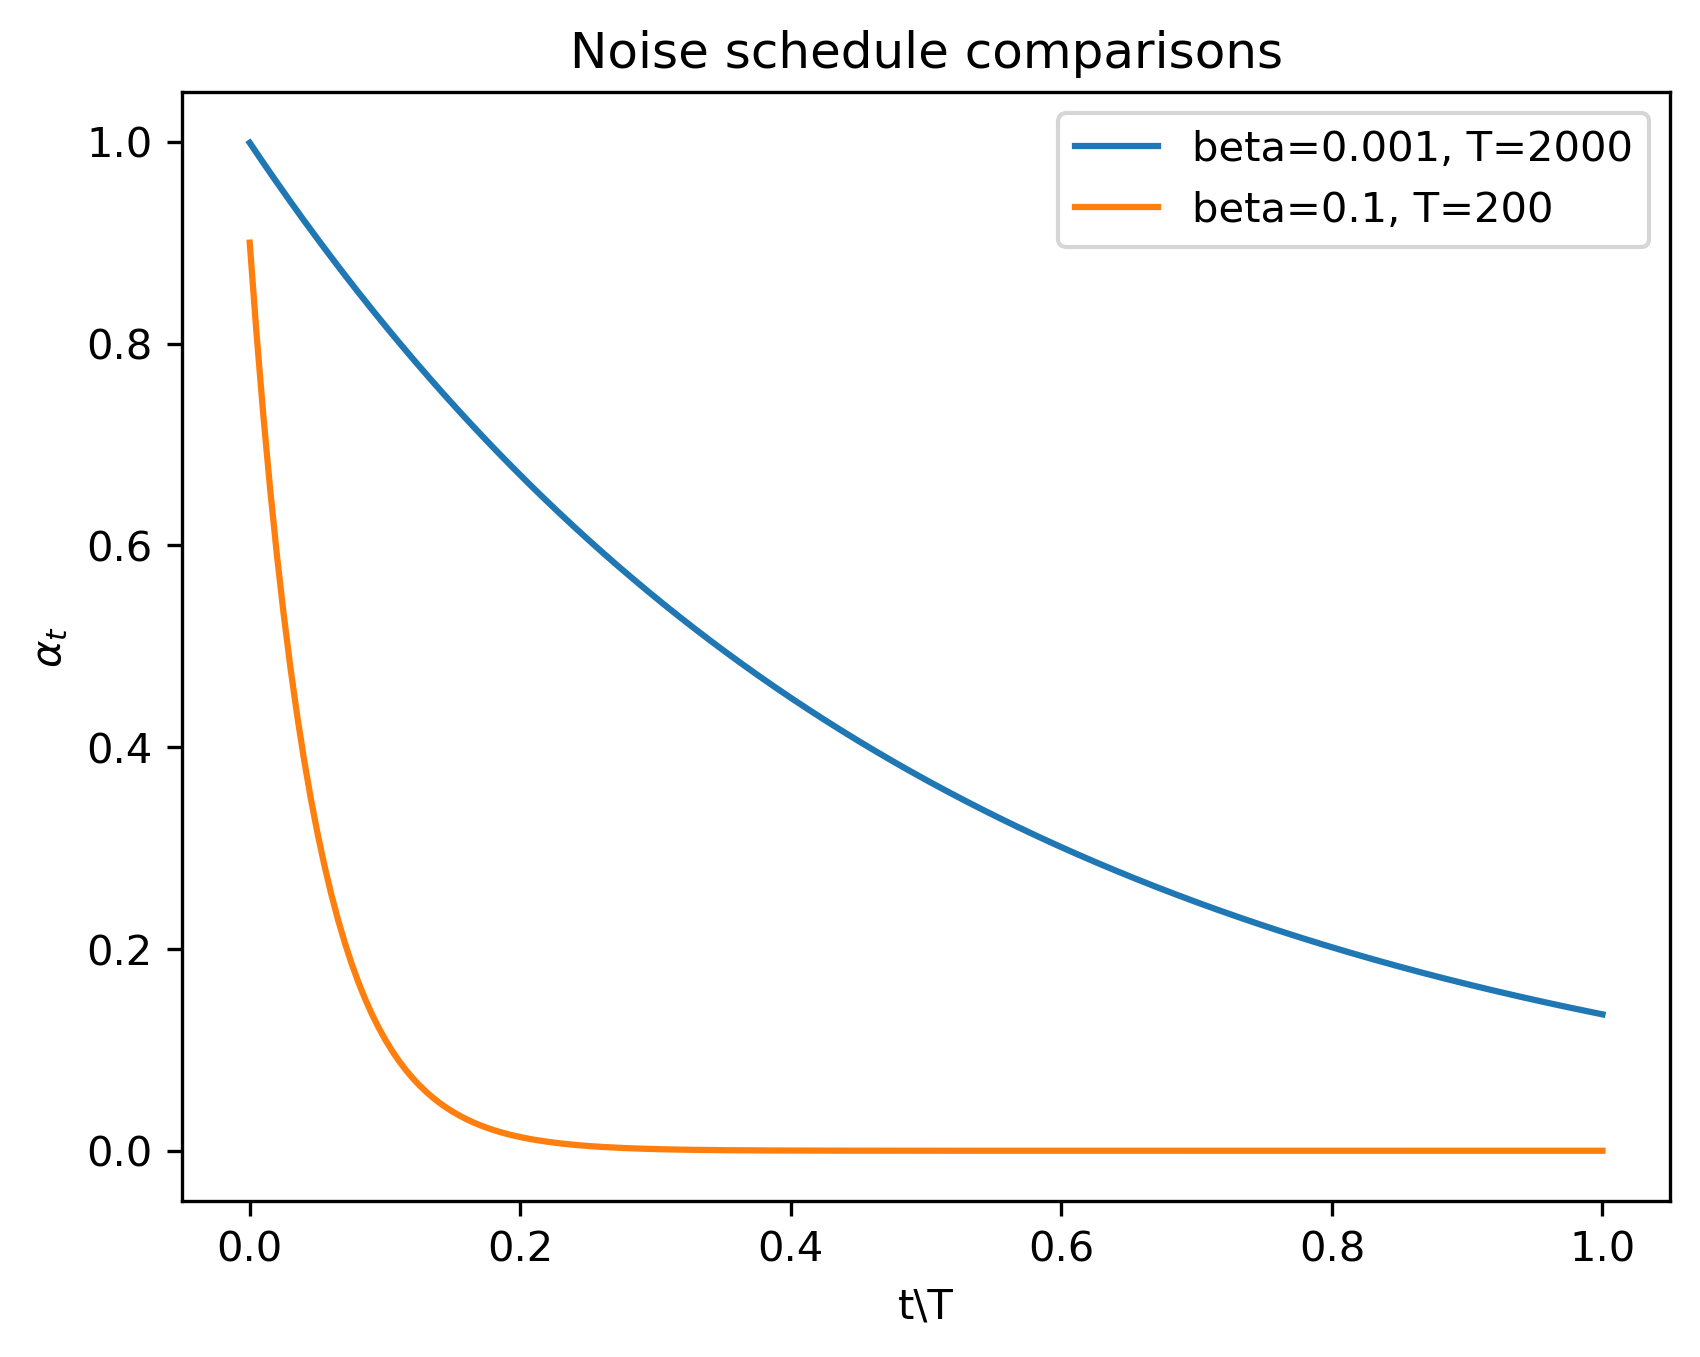
\includegraphics[width=0.5\textwidth]{figs/q1c_noise_schedule_comparison.png}
    \caption{Comparison of the noise schedules for the two models.}
    \label{fig:q1c_noise_schedules}
\end{figure}
Figure \ref{fig:q1c_noise_schedules} also reveals another interesting result. Even though the model with the smaller $\beta$ does not achieve an $\alpha_T$ value of zero (approximately 0.13), it still successfully generates high-quality samples with $Z_T$ sourced from a standard normal distribution. This indicates that one does not need to approximate the latent distribution $Pr(z_T)$ perfectly to generate high-quality samples. This will be further explored in the next section.

% Add direct reconstruction if space and time.


\section{Part 2 - Custom Degradatrion}
\subsection{Prelude - the UNet Decoder}
% Describe the modified decoder net
\subsection{The role of noise}
Add PDFs that follow from this defined in prince and the approximations.
Show how if the update scheme is no longer random, then the reverse distributions are just points.
So the derivation and the theory behind the loss function breaks down.
\subsection{The properties of D and R}

\bibliographystyle{plain}
\bibliography{ref.bib}
\end{document}


#NOTES ABOUT PART 2

Degradatrion must be smooth, without fixing eps model gave trash.
